\chapter{绪论}
\chaptermark{绪论}
	\section{研究背景}

	\subsection{人工智能的发展}
无孔不入的人工智能,别应用在各个领域,比如谷歌传统的搜索和广告业务、无人驾驶汽车,以及医疗健康部门,苹果Siri:为你解决问题的人工智能,应用了人工智能的百度外卖,代替人工顾问的智能应用,作为医疗辅助等。从互联网巨头到初创企业,都将人工智能作为发展的核心,如果关注这方面的新闻,应该看到过这样的一些新闻,"百度以近12亿元剥离游戏业务","央行成立金融科技委员会:用人工智能、云计算丰富监管手段",”苹果斥资2亿美元收购人工智能公司Lattice“等。人工智能变得越来越重要,两会期间,讯飞科大的语音识别及人工智能产品展示时,赢得了一众喝彩。 人工智能不仅涉及到民用,也涉及国家各个核心战略领域。国家主席习近平“一带一路“中演讲。他表示,“一带一路”建设要坚持创新驱动发展,加强在数字经济、人工智能、纳米技术、量子计算机等前沿领域的合作,推动大数据、云计算、智慧城市建设,连接成二十一世纪的数字丝绸之路。在这个人工智能到来的时代,发展人工智能变得越发重要。无论在国内国外,人工智能的发展都被寄予厚望。
	

		\subsection{深度学习的走红}
	随着人工智能的迅速走红,深度学习一词也迅速走红。人工智能是应用范畴的词汇,机器学习是一种实现人工智能的方法,深度学习是一种实现机器学习的方法,也是现有机器学习方法中,最奏效的一类。三者的关系见图1-1,人工智能是最外面的,下来是机器学习,最里面的是深度学习。而计算机视觉是机器学习应用最成功的一个方面,发展最为迅猛的一个分支。计算机视觉在很多方面都有应用,最为大家熟知的有人脸识别,组织恶意软件,语音识别,	无人驾驶汽车,在生物,医学方面也都有一定的应用,实际上,思科的一个评估显示,在2016年互联网上超过85\%的信息都会是像素形式,我们进入“多媒体”时代,视觉的时代,图片和视频的时代。由于互联网作为信息的载体,以及大量(视觉)传感器引发了视觉信息的大爆炸。CS231a深度学习与计算机视觉课程开篇,李菲菲教授讲计算机视觉(CV)她将这些视觉信息称为“互联网中的暗物质”,并且举了YouTube的一个例子,我们没法对这么大量的数据进行浏览,标记,分类,索引等,但是使用计算机视觉技术能够对照片进行标签、分类、处理视频中的每一帧,自动截取出篮球比赛中----比如说科比的一次精彩进球,我们现在面临着的问题就是,大量的数据,以及这些“暗物质”的挑战。目标识别与检测作为计算机视觉的一个应用,是很有应用价值的问题,而且是很多问题的根本解决之策。
	
		\subsection{TensorFlow的出现}	
	2015年11月,谷歌宣布TensorFlow开源,由于其灵活的架构可以在一个或多个CPU,GPU、桌面、服务器、以及移动设备上部署,还不用重新编写代码,其分布式计算的方法大大缩短了机器学习的训练时间,核心代码是C++编写的简化了线上部署的复杂度,还有Python、GO、Java的接口,用户可以很容易的使用,可视化的TensorBoard,极快的编译速度,并行计算模式等优点,使其作为一个开源软件库,刚开源第一个月就积累了10000+的star,而到现在star数已经到了56939, 是GitHub上最受欢迎的深度学习框架。在图形分类、音频处理、推荐系统和自然语言处理等场景下都有丰富的应用。最近流行的Keras框架底层默认使用TensorFlow,著名的斯坦福CS231n课程使用TensorFlow作为授课和作业的编程语言,而且现在除了谷歌内部大规模使用之外,优步(Uber)、Twitter、京东、小米、FaceBook等都在使用。TensorFlow的contrib.learn模块提供了一个让开发人员从scikit-learn或Keras进入到TensorFlow的桥梁,避免了从一个框架转移到另一个框架的无措感。TensorFlow的出现使更多对机器学习感兴趣的人可以去涉足这个领域,而不是因为电脑硬件的问题,机器学习训练时间过长的问题驻足。
	人工智能,机器学习,深度学习,TensorFlow成为越来越受欢迎的话题,我在百度指数,以及Google trends上,分别输入了机器学习,深度学习,还有人工智能几个搜索词后,得到的搜索热度趋势图见图1-2。通过这些数据得出的结论是人工智能,深度学习,正在变得越来重要,正在引起越来越多的重视。而在Google trends中看到TensorFlow搜索热度趋势图见图1-3 。TensorFlow的热度基本维持在100,足以说明这是目前很受欢迎的一个话题。
		\begin{figure}[p]
		\centering
		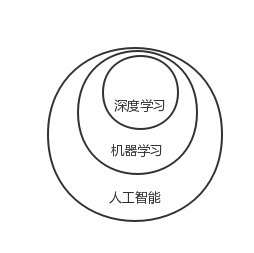
\includegraphics[width=0.7\linewidth]{figures/1-1}
		\caption[人工智能,机器学习,深度学习三者的关系图]{}
		\caption{}
		\label{fig:1-1}
	\end{figure}
	\begin{figure}[p]
		\centering
		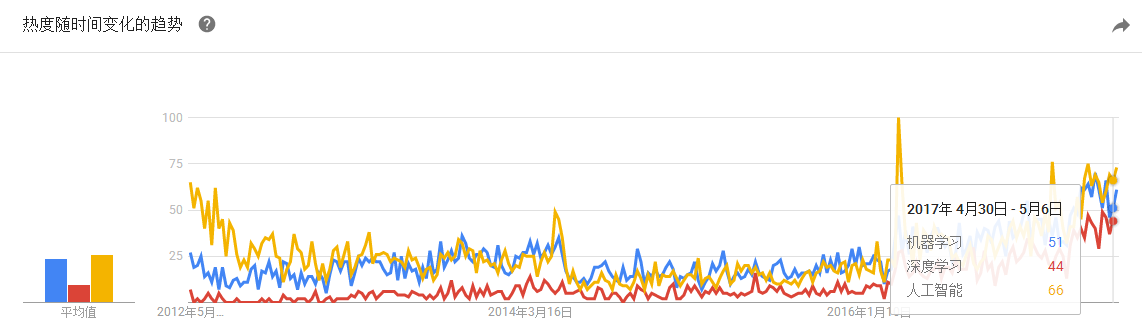
\includegraphics[width=0.5\linewidth]{figures/1-2}
		\caption{Google trends搜索热度趋势图:词汇的热度按0~100分为100个等级,可以看出来三者都呈上升趋势,并且相当的受欢迎。}
		\label{fig:1-2}
	\end{figure}
	\begin{figure}[p]
	\centering
	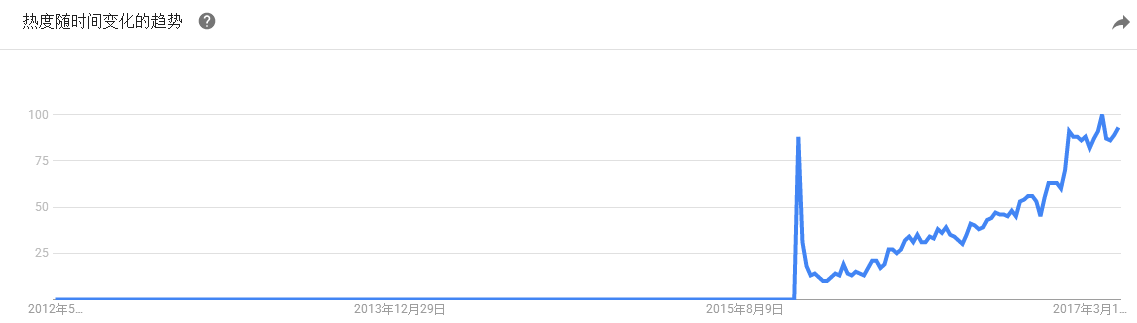
\includegraphics[width=0.5\linewidth]{figures/1-3}
	\caption[TensorFlow 在谷歌搜索的热度趋势]{}
	\caption{}
	\label{fig:1-3}
\end{figure}
\section{深度学习}
\subsection{}

		
	\section{本文研究内容}
		
		
	\section{本文内容安排}
	